% Created by tikzDevice version 0.12.3.1 on 2021-05-10 15:34:29
% !TEX encoding = UTF-8 Unicode
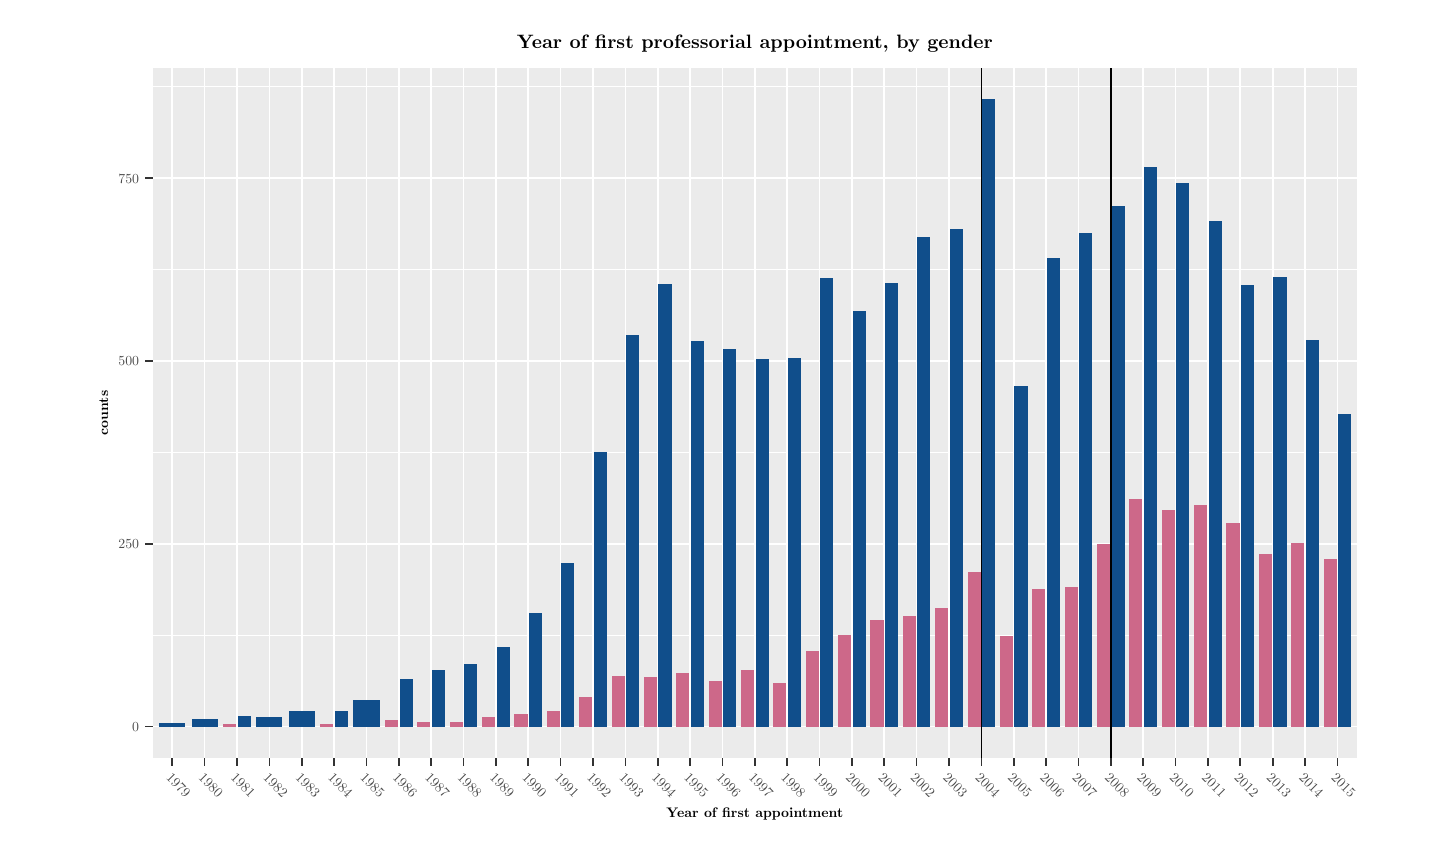
\begin{tikzpicture}[x=1pt,y=1pt]
\definecolor{fillColor}{RGB}{255,255,255}
\path[use as bounding box,fill=fillColor] (0,0) rectangle (505.89,289.08);
\begin{scope}
\path[clip] (  0.00,  0.00) rectangle (505.89,289.08);
\definecolor{drawColor}{RGB}{255,255,255}

\path[draw=drawColor,line width= 0.6pt,line join=round,line cap=round,fill=fillColor] (  0.00,  0.00) rectangle (505.89,289.08);
\end{scope}
\begin{scope}
\path[clip] ( 45.23, 25.16) rectangle (480.28,274.54);
\definecolor{fillColor}{gray}{0.92}

\path[fill=fillColor] ( 45.23, 25.16) rectangle (480.28,274.54);
\definecolor{drawColor}{RGB}{255,255,255}

\path[draw=drawColor,line width= 0.3pt,line join=round] ( 45.23, 69.52) --
	(480.28, 69.52);

\path[draw=drawColor,line width= 0.3pt,line join=round] ( 45.23,135.58) --
	(480.28,135.58);

\path[draw=drawColor,line width= 0.3pt,line join=round] ( 45.23,201.64) --
	(480.28,201.64);

\path[draw=drawColor,line width= 0.3pt,line join=round] ( 45.23,267.70) --
	(480.28,267.70);

\path[draw=drawColor,line width= 0.6pt,line join=round] ( 45.23, 36.50) --
	(480.28, 36.50);

\path[draw=drawColor,line width= 0.6pt,line join=round] ( 45.23,102.55) --
	(480.28,102.55);

\path[draw=drawColor,line width= 0.6pt,line join=round] ( 45.23,168.61) --
	(480.28,168.61);

\path[draw=drawColor,line width= 0.6pt,line join=round] ( 45.23,234.67) --
	(480.28,234.67);

\path[draw=drawColor,line width= 0.6pt,line join=round] ( 52.25, 25.16) --
	( 52.25,274.54);

\path[draw=drawColor,line width= 0.6pt,line join=round] ( 63.94, 25.16) --
	( 63.94,274.54);

\path[draw=drawColor,line width= 0.6pt,line join=round] ( 75.64, 25.16) --
	( 75.64,274.54);

\path[draw=drawColor,line width= 0.6pt,line join=round] ( 87.33, 25.16) --
	( 87.33,274.54);

\path[draw=drawColor,line width= 0.6pt,line join=round] ( 99.03, 25.16) --
	( 99.03,274.54);

\path[draw=drawColor,line width= 0.6pt,line join=round] (110.72, 25.16) --
	(110.72,274.54);

\path[draw=drawColor,line width= 0.6pt,line join=round] (122.42, 25.16) --
	(122.42,274.54);

\path[draw=drawColor,line width= 0.6pt,line join=round] (134.11, 25.16) --
	(134.11,274.54);

\path[draw=drawColor,line width= 0.6pt,line join=round] (145.81, 25.16) --
	(145.81,274.54);

\path[draw=drawColor,line width= 0.6pt,line join=round] (157.50, 25.16) --
	(157.50,274.54);

\path[draw=drawColor,line width= 0.6pt,line join=round] (169.20, 25.16) --
	(169.20,274.54);

\path[draw=drawColor,line width= 0.6pt,line join=round] (180.89, 25.16) --
	(180.89,274.54);

\path[draw=drawColor,line width= 0.6pt,line join=round] (192.59, 25.16) --
	(192.59,274.54);

\path[draw=drawColor,line width= 0.6pt,line join=round] (204.28, 25.16) --
	(204.28,274.54);

\path[draw=drawColor,line width= 0.6pt,line join=round] (215.98, 25.16) --
	(215.98,274.54);

\path[draw=drawColor,line width= 0.6pt,line join=round] (227.67, 25.16) --
	(227.67,274.54);

\path[draw=drawColor,line width= 0.6pt,line join=round] (239.37, 25.16) --
	(239.37,274.54);

\path[draw=drawColor,line width= 0.6pt,line join=round] (251.06, 25.16) --
	(251.06,274.54);

\path[draw=drawColor,line width= 0.6pt,line join=round] (262.76, 25.16) --
	(262.76,274.54);

\path[draw=drawColor,line width= 0.6pt,line join=round] (274.45, 25.16) --
	(274.45,274.54);

\path[draw=drawColor,line width= 0.6pt,line join=round] (286.15, 25.16) --
	(286.15,274.54);

\path[draw=drawColor,line width= 0.6pt,line join=round] (297.84, 25.16) --
	(297.84,274.54);

\path[draw=drawColor,line width= 0.6pt,line join=round] (309.54, 25.16) --
	(309.54,274.54);

\path[draw=drawColor,line width= 0.6pt,line join=round] (321.23, 25.16) --
	(321.23,274.54);

\path[draw=drawColor,line width= 0.6pt,line join=round] (332.93, 25.16) --
	(332.93,274.54);

\path[draw=drawColor,line width= 0.6pt,line join=round] (344.62, 25.16) --
	(344.62,274.54);

\path[draw=drawColor,line width= 0.6pt,line join=round] (356.32, 25.16) --
	(356.32,274.54);

\path[draw=drawColor,line width= 0.6pt,line join=round] (368.01, 25.16) --
	(368.01,274.54);

\path[draw=drawColor,line width= 0.6pt,line join=round] (379.71, 25.16) --
	(379.71,274.54);

\path[draw=drawColor,line width= 0.6pt,line join=round] (391.40, 25.16) --
	(391.40,274.54);

\path[draw=drawColor,line width= 0.6pt,line join=round] (403.10, 25.16) --
	(403.10,274.54);

\path[draw=drawColor,line width= 0.6pt,line join=round] (414.79, 25.16) --
	(414.79,274.54);

\path[draw=drawColor,line width= 0.6pt,line join=round] (426.49, 25.16) --
	(426.49,274.54);

\path[draw=drawColor,line width= 0.6pt,line join=round] (438.18, 25.16) --
	(438.18,274.54);

\path[draw=drawColor,line width= 0.6pt,line join=round] (449.88, 25.16) --
	(449.88,274.54);

\path[draw=drawColor,line width= 0.6pt,line join=round] (461.57, 25.16) --
	(461.57,274.54);

\path[draw=drawColor,line width= 0.6pt,line join=round] (473.27, 25.16) --
	(473.27,274.54);
\definecolor{fillColor}{RGB}{16,78,139}

\path[fill=fillColor] ( 47.51, 36.50) rectangle ( 56.98, 37.82);

\path[fill=fillColor] ( 59.20, 36.50) rectangle ( 68.68, 39.14);
\definecolor{fillColor}{RGB}{205,104,137}

\path[fill=fillColor] ( 70.64, 36.50) rectangle ( 75.37, 37.29);
\definecolor{fillColor}{RGB}{16,78,139}

\path[fill=fillColor] ( 75.90, 36.50) rectangle ( 80.63, 40.46);

\path[fill=fillColor] ( 82.59, 36.50) rectangle ( 92.07, 39.93);

\path[fill=fillColor] ( 94.29, 36.50) rectangle (103.76, 42.31);
\definecolor{fillColor}{RGB}{205,104,137}

\path[fill=fillColor] (105.72, 36.50) rectangle (110.46, 37.29);
\definecolor{fillColor}{RGB}{16,78,139}

\path[fill=fillColor] (110.98, 36.50) rectangle (115.72, 42.04);

\path[fill=fillColor] (117.68, 36.50) rectangle (127.15, 46.01);
\definecolor{fillColor}{RGB}{205,104,137}

\path[fill=fillColor] (129.11, 36.50) rectangle (133.85, 38.87);
\definecolor{fillColor}{RGB}{16,78,139}

\path[fill=fillColor] (134.37, 36.50) rectangle (139.11, 53.67);
\definecolor{fillColor}{RGB}{205,104,137}

\path[fill=fillColor] (140.81, 36.50) rectangle (145.54, 38.34);
\definecolor{fillColor}{RGB}{16,78,139}

\path[fill=fillColor] (146.07, 36.50) rectangle (150.80, 57.11);
\definecolor{fillColor}{RGB}{205,104,137}

\path[fill=fillColor] (152.50, 36.50) rectangle (157.24, 38.34);
\definecolor{fillColor}{RGB}{16,78,139}

\path[fill=fillColor] (157.76, 36.50) rectangle (162.50, 59.22);
\definecolor{fillColor}{RGB}{205,104,137}

\path[fill=fillColor] (164.20, 36.50) rectangle (168.93, 39.93);
\definecolor{fillColor}{RGB}{16,78,139}

\path[fill=fillColor] (169.46, 36.50) rectangle (174.19, 65.30);
\definecolor{fillColor}{RGB}{205,104,137}

\path[fill=fillColor] (175.89, 36.50) rectangle (180.63, 40.99);
\definecolor{fillColor}{RGB}{16,78,139}

\path[fill=fillColor] (181.15, 36.50) rectangle (185.89, 77.72);
\definecolor{fillColor}{RGB}{205,104,137}

\path[fill=fillColor] (187.59, 36.50) rectangle (192.32, 42.31);
\definecolor{fillColor}{RGB}{16,78,139}

\path[fill=fillColor] (192.85, 36.50) rectangle (197.58, 95.68);
\definecolor{fillColor}{RGB}{205,104,137}

\path[fill=fillColor] (199.28, 36.50) rectangle (204.02, 47.33);
\definecolor{fillColor}{RGB}{16,78,139}

\path[fill=fillColor] (204.54, 36.50) rectangle (209.28,135.85);
\definecolor{fillColor}{RGB}{205,104,137}

\path[fill=fillColor] (210.98, 36.50) rectangle (215.71, 54.73);
\definecolor{fillColor}{RGB}{16,78,139}

\path[fill=fillColor] (216.24, 36.50) rectangle (220.97,177.86);
\definecolor{fillColor}{RGB}{205,104,137}

\path[fill=fillColor] (222.67, 36.50) rectangle (227.41, 54.46);
\definecolor{fillColor}{RGB}{16,78,139}

\path[fill=fillColor] (227.93, 36.50) rectangle (232.67,196.62);
\definecolor{fillColor}{RGB}{205,104,137}

\path[fill=fillColor] (234.37, 36.50) rectangle (239.10, 56.05);
\definecolor{fillColor}{RGB}{16,78,139}

\path[fill=fillColor] (239.63, 36.50) rectangle (244.36,175.75);
\definecolor{fillColor}{RGB}{205,104,137}

\path[fill=fillColor] (246.06, 36.50) rectangle (250.80, 52.88);
\definecolor{fillColor}{RGB}{16,78,139}

\path[fill=fillColor] (251.32, 36.50) rectangle (256.06,173.10);
\definecolor{fillColor}{RGB}{205,104,137}

\path[fill=fillColor] (257.76, 36.50) rectangle (262.49, 57.11);
\definecolor{fillColor}{RGB}{16,78,139}

\path[fill=fillColor] (263.02, 36.50) rectangle (267.75,169.40);
\definecolor{fillColor}{RGB}{205,104,137}

\path[fill=fillColor] (269.45, 36.50) rectangle (274.19, 52.35);
\definecolor{fillColor}{RGB}{16,78,139}

\path[fill=fillColor] (274.71, 36.50) rectangle (279.45,169.67);
\definecolor{fillColor}{RGB}{205,104,137}

\path[fill=fillColor] (281.15, 36.50) rectangle (285.88, 63.98);
\definecolor{fillColor}{RGB}{16,78,139}

\path[fill=fillColor] (286.41, 36.50) rectangle (291.14,198.73);
\definecolor{fillColor}{RGB}{205,104,137}

\path[fill=fillColor] (292.84, 36.50) rectangle (297.58, 69.52);
\definecolor{fillColor}{RGB}{16,78,139}

\path[fill=fillColor] (298.10, 36.50) rectangle (302.84,186.58);
\definecolor{fillColor}{RGB}{205,104,137}

\path[fill=fillColor] (304.54, 36.50) rectangle (309.27, 75.07);
\definecolor{fillColor}{RGB}{16,78,139}

\path[fill=fillColor] (309.80, 36.50) rectangle (314.54,196.88);
\definecolor{fillColor}{RGB}{205,104,137}

\path[fill=fillColor] (316.23, 36.50) rectangle (320.97, 76.39);
\definecolor{fillColor}{RGB}{16,78,139}

\path[fill=fillColor] (321.49, 36.50) rectangle (326.23,213.53);
\definecolor{fillColor}{RGB}{205,104,137}

\path[fill=fillColor] (327.93, 36.50) rectangle (332.66, 79.30);
\definecolor{fillColor}{RGB}{16,78,139}

\path[fill=fillColor] (333.19, 36.50) rectangle (337.93,216.17);
\definecolor{fillColor}{RGB}{205,104,137}

\path[fill=fillColor] (339.62, 36.50) rectangle (344.36, 92.25);
\definecolor{fillColor}{RGB}{16,78,139}

\path[fill=fillColor] (344.88, 36.50) rectangle (349.62,263.21);
\definecolor{fillColor}{RGB}{205,104,137}

\path[fill=fillColor] (351.32, 36.50) rectangle (356.05, 69.26);
\definecolor{fillColor}{RGB}{16,78,139}

\path[fill=fillColor] (356.58, 36.50) rectangle (361.32,159.63);
\definecolor{fillColor}{RGB}{205,104,137}

\path[fill=fillColor] (363.01, 36.50) rectangle (367.75, 86.17);
\definecolor{fillColor}{RGB}{16,78,139}

\path[fill=fillColor] (368.27, 36.50) rectangle (373.01,205.87);
\definecolor{fillColor}{RGB}{205,104,137}

\path[fill=fillColor] (374.71, 36.50) rectangle (379.44, 86.96);
\definecolor{fillColor}{RGB}{16,78,139}

\path[fill=fillColor] (379.97, 36.50) rectangle (384.71,214.85);
\definecolor{fillColor}{RGB}{205,104,137}

\path[fill=fillColor] (386.40, 36.50) rectangle (391.14,102.55);
\definecolor{fillColor}{RGB}{16,78,139}

\path[fill=fillColor] (391.66, 36.50) rectangle (396.40,224.63);
\definecolor{fillColor}{RGB}{205,104,137}

\path[fill=fillColor] (398.10, 36.50) rectangle (402.83,118.94);
\definecolor{fillColor}{RGB}{16,78,139}

\path[fill=fillColor] (403.36, 36.50) rectangle (408.10,238.90);
\definecolor{fillColor}{RGB}{205,104,137}

\path[fill=fillColor] (409.79, 36.50) rectangle (414.53,114.71);
\definecolor{fillColor}{RGB}{16,78,139}

\path[fill=fillColor] (415.05, 36.50) rectangle (419.79,232.82);
\definecolor{fillColor}{RGB}{205,104,137}

\path[fill=fillColor] (421.49, 36.50) rectangle (426.22,116.56);
\definecolor{fillColor}{RGB}{16,78,139}

\path[fill=fillColor] (426.75, 36.50) rectangle (431.49,219.34);
\definecolor{fillColor}{RGB}{205,104,137}

\path[fill=fillColor] (433.18, 36.50) rectangle (437.92,110.22);
\definecolor{fillColor}{RGB}{16,78,139}

\path[fill=fillColor] (438.44, 36.50) rectangle (443.18,196.09);
\definecolor{fillColor}{RGB}{205,104,137}

\path[fill=fillColor] (444.88, 36.50) rectangle (449.61, 98.85);
\definecolor{fillColor}{RGB}{16,78,139}

\path[fill=fillColor] (450.14, 36.50) rectangle (454.88,199.00);
\definecolor{fillColor}{RGB}{205,104,137}

\path[fill=fillColor] (456.57, 36.50) rectangle (461.31,102.82);
\definecolor{fillColor}{RGB}{16,78,139}

\path[fill=fillColor] (461.83, 36.50) rectangle (466.57,176.27);
\definecolor{fillColor}{RGB}{205,104,137}

\path[fill=fillColor] (468.27, 36.50) rectangle (473.00, 97.00);
\definecolor{fillColor}{RGB}{16,78,139}

\path[fill=fillColor] (473.53, 36.50) rectangle (478.27,149.59);
\definecolor{drawColor}{RGB}{0,0,0}

\path[draw=drawColor,line width= 0.6pt,line join=round] (344.62, 25.16) -- (344.62,274.54);

\path[draw=drawColor,line width= 0.6pt,line join=round] (391.40, 25.16) -- (391.40,274.54);
\end{scope}
\begin{scope}
\path[clip] (  0.00,  0.00) rectangle (505.89,289.08);
\definecolor{drawColor}{gray}{0.30}

\node[text=drawColor,anchor=base east,inner sep=0pt, outer sep=0pt, scale=  0.50] at ( 40.28, 34.77) {0};

\node[text=drawColor,anchor=base east,inner sep=0pt, outer sep=0pt, scale=  0.50] at ( 40.28,100.83) {250};

\node[text=drawColor,anchor=base east,inner sep=0pt, outer sep=0pt, scale=  0.50] at ( 40.28,166.89) {500};

\node[text=drawColor,anchor=base east,inner sep=0pt, outer sep=0pt, scale=  0.50] at ( 40.28,232.95) {750};
\end{scope}
\begin{scope}
\path[clip] (  0.00,  0.00) rectangle (505.89,289.08);
\definecolor{drawColor}{gray}{0.20}

\path[draw=drawColor,line width= 0.6pt,line join=round] ( 42.48, 36.50) --
	( 45.23, 36.50);

\path[draw=drawColor,line width= 0.6pt,line join=round] ( 42.48,102.55) --
	( 45.23,102.55);

\path[draw=drawColor,line width= 0.6pt,line join=round] ( 42.48,168.61) --
	( 45.23,168.61);

\path[draw=drawColor,line width= 0.6pt,line join=round] ( 42.48,234.67) --
	( 45.23,234.67);
\end{scope}
\begin{scope}
\path[clip] (  0.00,  0.00) rectangle (505.89,289.08);
\definecolor{drawColor}{gray}{0.20}

\path[draw=drawColor,line width= 0.6pt,line join=round] ( 52.25, 22.41) --
	( 52.25, 25.16);

\path[draw=drawColor,line width= 0.6pt,line join=round] ( 63.94, 22.41) --
	( 63.94, 25.16);

\path[draw=drawColor,line width= 0.6pt,line join=round] ( 75.64, 22.41) --
	( 75.64, 25.16);

\path[draw=drawColor,line width= 0.6pt,line join=round] ( 87.33, 22.41) --
	( 87.33, 25.16);

\path[draw=drawColor,line width= 0.6pt,line join=round] ( 99.03, 22.41) --
	( 99.03, 25.16);

\path[draw=drawColor,line width= 0.6pt,line join=round] (110.72, 22.41) --
	(110.72, 25.16);

\path[draw=drawColor,line width= 0.6pt,line join=round] (122.42, 22.41) --
	(122.42, 25.16);

\path[draw=drawColor,line width= 0.6pt,line join=round] (134.11, 22.41) --
	(134.11, 25.16);

\path[draw=drawColor,line width= 0.6pt,line join=round] (145.81, 22.41) --
	(145.81, 25.16);

\path[draw=drawColor,line width= 0.6pt,line join=round] (157.50, 22.41) --
	(157.50, 25.16);

\path[draw=drawColor,line width= 0.6pt,line join=round] (169.20, 22.41) --
	(169.20, 25.16);

\path[draw=drawColor,line width= 0.6pt,line join=round] (180.89, 22.41) --
	(180.89, 25.16);

\path[draw=drawColor,line width= 0.6pt,line join=round] (192.59, 22.41) --
	(192.59, 25.16);

\path[draw=drawColor,line width= 0.6pt,line join=round] (204.28, 22.41) --
	(204.28, 25.16);

\path[draw=drawColor,line width= 0.6pt,line join=round] (215.98, 22.41) --
	(215.98, 25.16);

\path[draw=drawColor,line width= 0.6pt,line join=round] (227.67, 22.41) --
	(227.67, 25.16);

\path[draw=drawColor,line width= 0.6pt,line join=round] (239.37, 22.41) --
	(239.37, 25.16);

\path[draw=drawColor,line width= 0.6pt,line join=round] (251.06, 22.41) --
	(251.06, 25.16);

\path[draw=drawColor,line width= 0.6pt,line join=round] (262.76, 22.41) --
	(262.76, 25.16);

\path[draw=drawColor,line width= 0.6pt,line join=round] (274.45, 22.41) --
	(274.45, 25.16);

\path[draw=drawColor,line width= 0.6pt,line join=round] (286.15, 22.41) --
	(286.15, 25.16);

\path[draw=drawColor,line width= 0.6pt,line join=round] (297.84, 22.41) --
	(297.84, 25.16);

\path[draw=drawColor,line width= 0.6pt,line join=round] (309.54, 22.41) --
	(309.54, 25.16);

\path[draw=drawColor,line width= 0.6pt,line join=round] (321.23, 22.41) --
	(321.23, 25.16);

\path[draw=drawColor,line width= 0.6pt,line join=round] (332.93, 22.41) --
	(332.93, 25.16);

\path[draw=drawColor,line width= 0.6pt,line join=round] (344.62, 22.41) --
	(344.62, 25.16);

\path[draw=drawColor,line width= 0.6pt,line join=round] (356.32, 22.41) --
	(356.32, 25.16);

\path[draw=drawColor,line width= 0.6pt,line join=round] (368.01, 22.41) --
	(368.01, 25.16);

\path[draw=drawColor,line width= 0.6pt,line join=round] (379.71, 22.41) --
	(379.71, 25.16);

\path[draw=drawColor,line width= 0.6pt,line join=round] (391.40, 22.41) --
	(391.40, 25.16);

\path[draw=drawColor,line width= 0.6pt,line join=round] (403.10, 22.41) --
	(403.10, 25.16);

\path[draw=drawColor,line width= 0.6pt,line join=round] (414.79, 22.41) --
	(414.79, 25.16);

\path[draw=drawColor,line width= 0.6pt,line join=round] (426.49, 22.41) --
	(426.49, 25.16);

\path[draw=drawColor,line width= 0.6pt,line join=round] (438.18, 22.41) --
	(438.18, 25.16);

\path[draw=drawColor,line width= 0.6pt,line join=round] (449.88, 22.41) --
	(449.88, 25.16);

\path[draw=drawColor,line width= 0.6pt,line join=round] (461.57, 22.41) --
	(461.57, 25.16);

\path[draw=drawColor,line width= 0.6pt,line join=round] (473.27, 22.41) --
	(473.27, 25.16);
\end{scope}
\begin{scope}
\path[clip] (  0.00,  0.00) rectangle (505.89,289.08);
\definecolor{drawColor}{gray}{0.30}

\node[text=drawColor,rotate=-45.00,anchor=base west,inner sep=0pt, outer sep=0pt, scale=  0.50] at ( 49.81, 17.77) {1979};

\node[text=drawColor,rotate=-45.00,anchor=base west,inner sep=0pt, outer sep=0pt, scale=  0.50] at ( 61.51, 17.77) {1980};

\node[text=drawColor,rotate=-45.00,anchor=base west,inner sep=0pt, outer sep=0pt, scale=  0.50] at ( 73.20, 17.77) {1981};

\node[text=drawColor,rotate=-45.00,anchor=base west,inner sep=0pt, outer sep=0pt, scale=  0.50] at ( 84.90, 17.77) {1982};

\node[text=drawColor,rotate=-45.00,anchor=base west,inner sep=0pt, outer sep=0pt, scale=  0.50] at ( 96.59, 17.77) {1983};

\node[text=drawColor,rotate=-45.00,anchor=base west,inner sep=0pt, outer sep=0pt, scale=  0.50] at (108.29, 17.77) {1984};

\node[text=drawColor,rotate=-45.00,anchor=base west,inner sep=0pt, outer sep=0pt, scale=  0.50] at (119.98, 17.77) {1985};

\node[text=drawColor,rotate=-45.00,anchor=base west,inner sep=0pt, outer sep=0pt, scale=  0.50] at (131.68, 17.77) {1986};

\node[text=drawColor,rotate=-45.00,anchor=base west,inner sep=0pt, outer sep=0pt, scale=  0.50] at (143.37, 17.77) {1987};

\node[text=drawColor,rotate=-45.00,anchor=base west,inner sep=0pt, outer sep=0pt, scale=  0.50] at (155.07, 17.77) {1988};

\node[text=drawColor,rotate=-45.00,anchor=base west,inner sep=0pt, outer sep=0pt, scale=  0.50] at (166.76, 17.77) {1989};

\node[text=drawColor,rotate=-45.00,anchor=base west,inner sep=0pt, outer sep=0pt, scale=  0.50] at (178.46, 17.77) {1990};

\node[text=drawColor,rotate=-45.00,anchor=base west,inner sep=0pt, outer sep=0pt, scale=  0.50] at (190.15, 17.77) {1991};

\node[text=drawColor,rotate=-45.00,anchor=base west,inner sep=0pt, outer sep=0pt, scale=  0.50] at (201.85, 17.77) {1992};

\node[text=drawColor,rotate=-45.00,anchor=base west,inner sep=0pt, outer sep=0pt, scale=  0.50] at (213.54, 17.77) {1993};

\node[text=drawColor,rotate=-45.00,anchor=base west,inner sep=0pt, outer sep=0pt, scale=  0.50] at (225.24, 17.77) {1994};

\node[text=drawColor,rotate=-45.00,anchor=base west,inner sep=0pt, outer sep=0pt, scale=  0.50] at (236.93, 17.77) {1995};

\node[text=drawColor,rotate=-45.00,anchor=base west,inner sep=0pt, outer sep=0pt, scale=  0.50] at (248.63, 17.77) {1996};

\node[text=drawColor,rotate=-45.00,anchor=base west,inner sep=0pt, outer sep=0pt, scale=  0.50] at (260.32, 17.77) {1997};

\node[text=drawColor,rotate=-45.00,anchor=base west,inner sep=0pt, outer sep=0pt, scale=  0.50] at (272.02, 17.77) {1998};

\node[text=drawColor,rotate=-45.00,anchor=base west,inner sep=0pt, outer sep=0pt, scale=  0.50] at (283.71, 17.77) {1999};

\node[text=drawColor,rotate=-45.00,anchor=base west,inner sep=0pt, outer sep=0pt, scale=  0.50] at (295.41, 17.77) {2000};

\node[text=drawColor,rotate=-45.00,anchor=base west,inner sep=0pt, outer sep=0pt, scale=  0.50] at (307.10, 17.77) {2001};

\node[text=drawColor,rotate=-45.00,anchor=base west,inner sep=0pt, outer sep=0pt, scale=  0.50] at (318.80, 17.77) {2002};

\node[text=drawColor,rotate=-45.00,anchor=base west,inner sep=0pt, outer sep=0pt, scale=  0.50] at (330.49, 17.77) {2003};

\node[text=drawColor,rotate=-45.00,anchor=base west,inner sep=0pt, outer sep=0pt, scale=  0.50] at (342.19, 17.77) {2004};

\node[text=drawColor,rotate=-45.00,anchor=base west,inner sep=0pt, outer sep=0pt, scale=  0.50] at (353.88, 17.77) {2005};

\node[text=drawColor,rotate=-45.00,anchor=base west,inner sep=0pt, outer sep=0pt, scale=  0.50] at (365.58, 17.77) {2006};

\node[text=drawColor,rotate=-45.00,anchor=base west,inner sep=0pt, outer sep=0pt, scale=  0.50] at (377.27, 17.77) {2007};

\node[text=drawColor,rotate=-45.00,anchor=base west,inner sep=0pt, outer sep=0pt, scale=  0.50] at (388.97, 17.77) {2008};

\node[text=drawColor,rotate=-45.00,anchor=base west,inner sep=0pt, outer sep=0pt, scale=  0.50] at (400.66, 17.77) {2009};

\node[text=drawColor,rotate=-45.00,anchor=base west,inner sep=0pt, outer sep=0pt, scale=  0.50] at (412.36, 17.77) {2010};

\node[text=drawColor,rotate=-45.00,anchor=base west,inner sep=0pt, outer sep=0pt, scale=  0.50] at (424.05, 17.77) {2011};

\node[text=drawColor,rotate=-45.00,anchor=base west,inner sep=0pt, outer sep=0pt, scale=  0.50] at (435.75, 17.77) {2012};

\node[text=drawColor,rotate=-45.00,anchor=base west,inner sep=0pt, outer sep=0pt, scale=  0.50] at (447.44, 17.77) {2013};

\node[text=drawColor,rotate=-45.00,anchor=base west,inner sep=0pt, outer sep=0pt, scale=  0.50] at (459.14, 17.77) {2014};

\node[text=drawColor,rotate=-45.00,anchor=base west,inner sep=0pt, outer sep=0pt, scale=  0.50] at (470.83, 17.77) {2015};
\end{scope}
\begin{scope}
\path[clip] (  0.00,  0.00) rectangle (505.89,289.08);
\definecolor{drawColor}{RGB}{0,0,0}

\node[text=drawColor,anchor=base,inner sep=0pt, outer sep=0pt, scale=  0.50] at (262.76,  3.82) {\bfseries Year of first appointment};
\end{scope}
\begin{scope}
\path[clip] (  0.00,  0.00) rectangle (505.89,289.08);
\definecolor{drawColor}{RGB}{0,0,0}

\node[text=drawColor,rotate= 90.00,anchor=base,inner sep=0pt, outer sep=0pt, scale=  0.50] at ( 29.06,149.85) {\bfseries counts};
\end{scope}
\begin{scope}
\path[clip] (  0.00,  0.00) rectangle (505.89,289.08);
\definecolor{drawColor}{RGB}{0,0,0}

\node[text=drawColor,anchor=base,inner sep=0pt, outer sep=0pt, scale=  0.70] at (262.76,281.40) {\bfseries Year of first professorial appointment, by gender};
\end{scope}
\end{tikzpicture}
